\subsection{POMDP-based Statistical Spoken Dialogue Systems: a Review \cite{Young2013Pomdp}}

By including an explicit Bayesian model of uncertainty and by optimising the policy via a reward-driven process, \emph{partially observable Markov decision processes (POMDPs)} provide a data-driven framework that reduces the cost of hand-crafting dialog managers and provides robustness against the errors created by speech recognisers operating in noisy environments. This paper provides an overview of the current state of the art in the development of \emph{POMDP-based spoken dialog systems (SDS)}.

\begin{figure}[htbp]
  \centering
  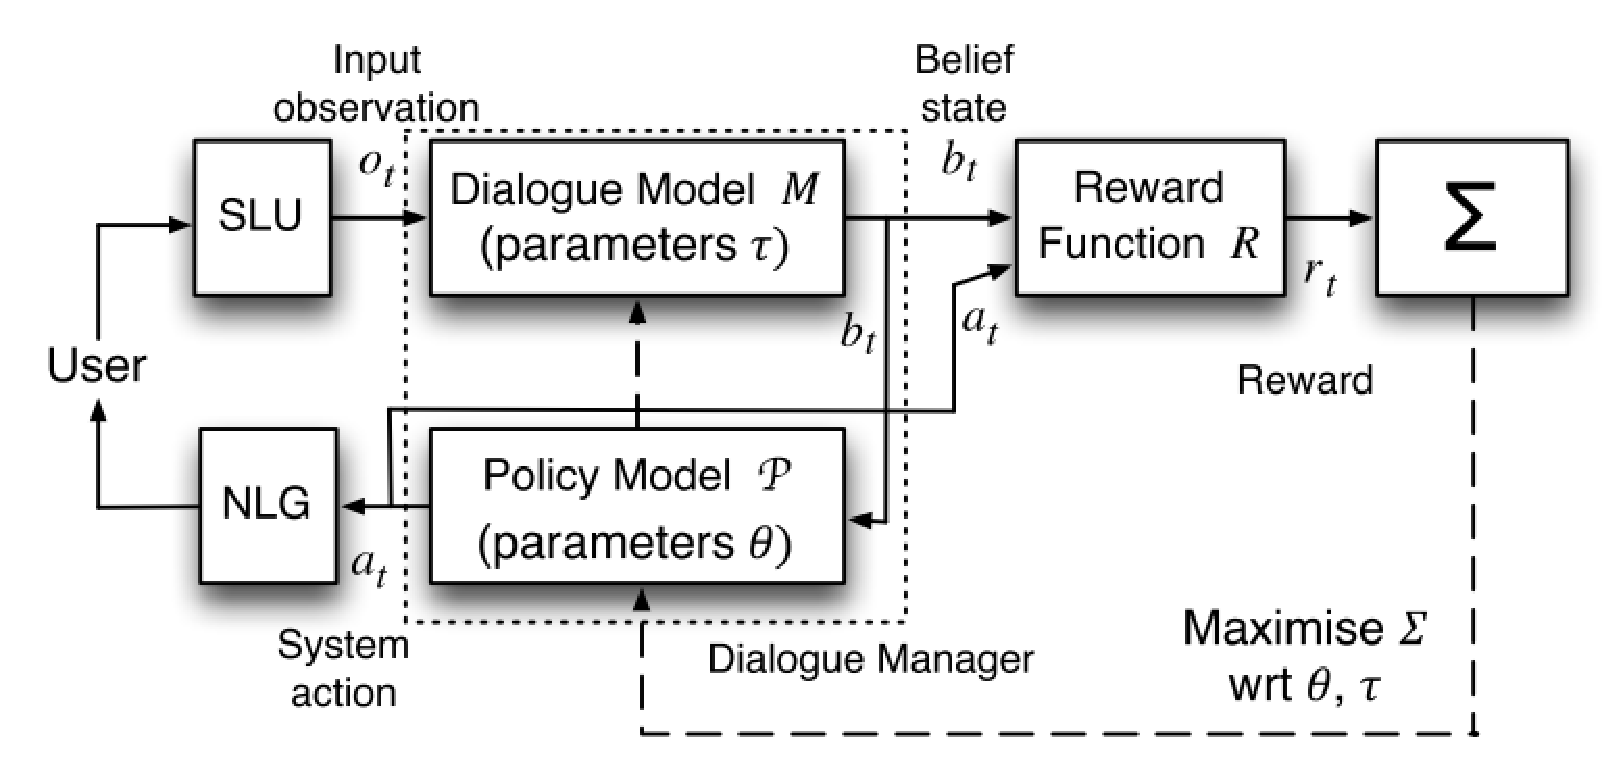
\includegraphics[width=.7\linewidth]{10_17_POMDP1}\\
  \caption{Components of a POMDP-based spoken dialog system}\label{fig:POMDP1}
\end{figure}

%The principal elements of a conventional Spoken Dialog System (SDS) are shown in Figure \ref.
The POMDP approach assumes that dialog evolves as a Markov process, i.e., starting in some initial state, each subsequent state is modelled by a transition probability $p(s_t | s_{t-1}, a_{t-1})$. The state $s_t$ is not directly observable. At each turn, the system regards the output of the SLU as a noisy observation $o_t$ of the user input with probability $p(o_t | s_t)$. The transition and observation probability functions are represented by the dialog model. The decision as to which action to take is represented by the policy. The components of a POMDP-based system are presented in Figure \ref{fig:POMDP1}.

\begin{figure}[htbp]
  \centering
  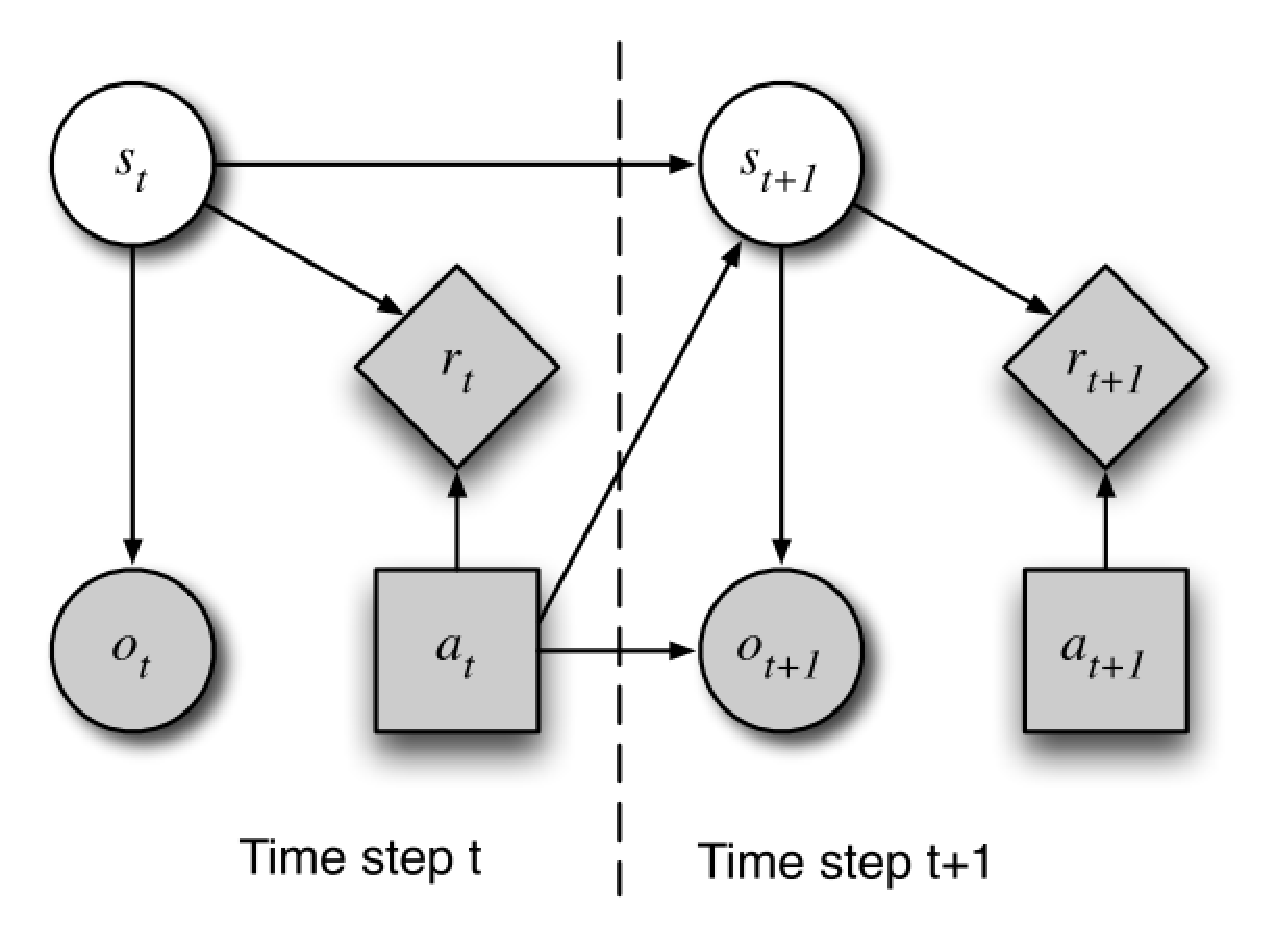
\includegraphics[width=.5\linewidth]{10_17_POMDP2}\\
  \caption{An influence diagram of a POMDP}\label{fig:POMDP2}
\end{figure}

The paper first introduces some preliminary knowledge about the POMDP method. In a POMDP system in each step the world is in some unobserved state $s_t$. Since $s_t$ is not known exactly, a distribution over possible states called a belief state $b_t$ is maintained, where $b_t(s_t)$ indicates the probability of being in a particular state $s_t$. Based on $b_t$, the machine selects an action $a_t$, receives a reward $r_t$, and transitions to (unobserved) state $s_{t+1}$. The machine then receives an observation $o_{t+1}$. This process is represented as an influence diagram in Figure \ref{fig:POMDP2}.

Given an existing belief state $b_t$, the last system action $a_t$, and a new observation $o_{t+1}$, the new updated belief state is given by:
$$b_{t+1}(s_{t+1}) = \eta P(o_{t+1} | s_{t+1}, a_t) \sum_{s_t} P(s_{t+1} | s_t, a_t)  b_t(s_t),$$
where $\eta$ is a normalization constant. The system action is determined by a policy $\pi$. The discounted sum of rewards expected by starting in $b_t$ and following policy $\pi$ is given by the value function $V^\pi(b_t)$. In POMDP, finding an optimal policy is called solving or optimizing the POMDP. However, standard POMDP methods do not scale to the complexity needed to represent a real-world dialog system. So the next sections of this paper introduce some domain-specific methods for applying POMDP in the SDS task.

The first step is to review some possible approaches to represent the dialog model. In a goal-oriented SDS, the state should encode three distinct types of information: the user's goal $g_t$, the intent of the most recent user utterance $u_t$, and the dialog history $h_t$. The resulting influence diagram is shown in Figure \ref{fig:POMDP2}, in which some reasonable independence assumptions have been introduced. Factoring the state in this way can significantly reduce the POMDP model complexity. However, it is still too complex to support tractable real-world systems, so further approximation is necessary. The paper introduces two main approaches: the N-best approach, and the factored Bayesian Network approach.

In N-best approaches, the belief state is approximated by a list of the most likely states with their probabilities. It can also be viewed as running N conventional dialog systems in parallel, such that each parallel thread tracks a different interpretation of what the user said.

\begin{figure}[htbp]
  \centering
  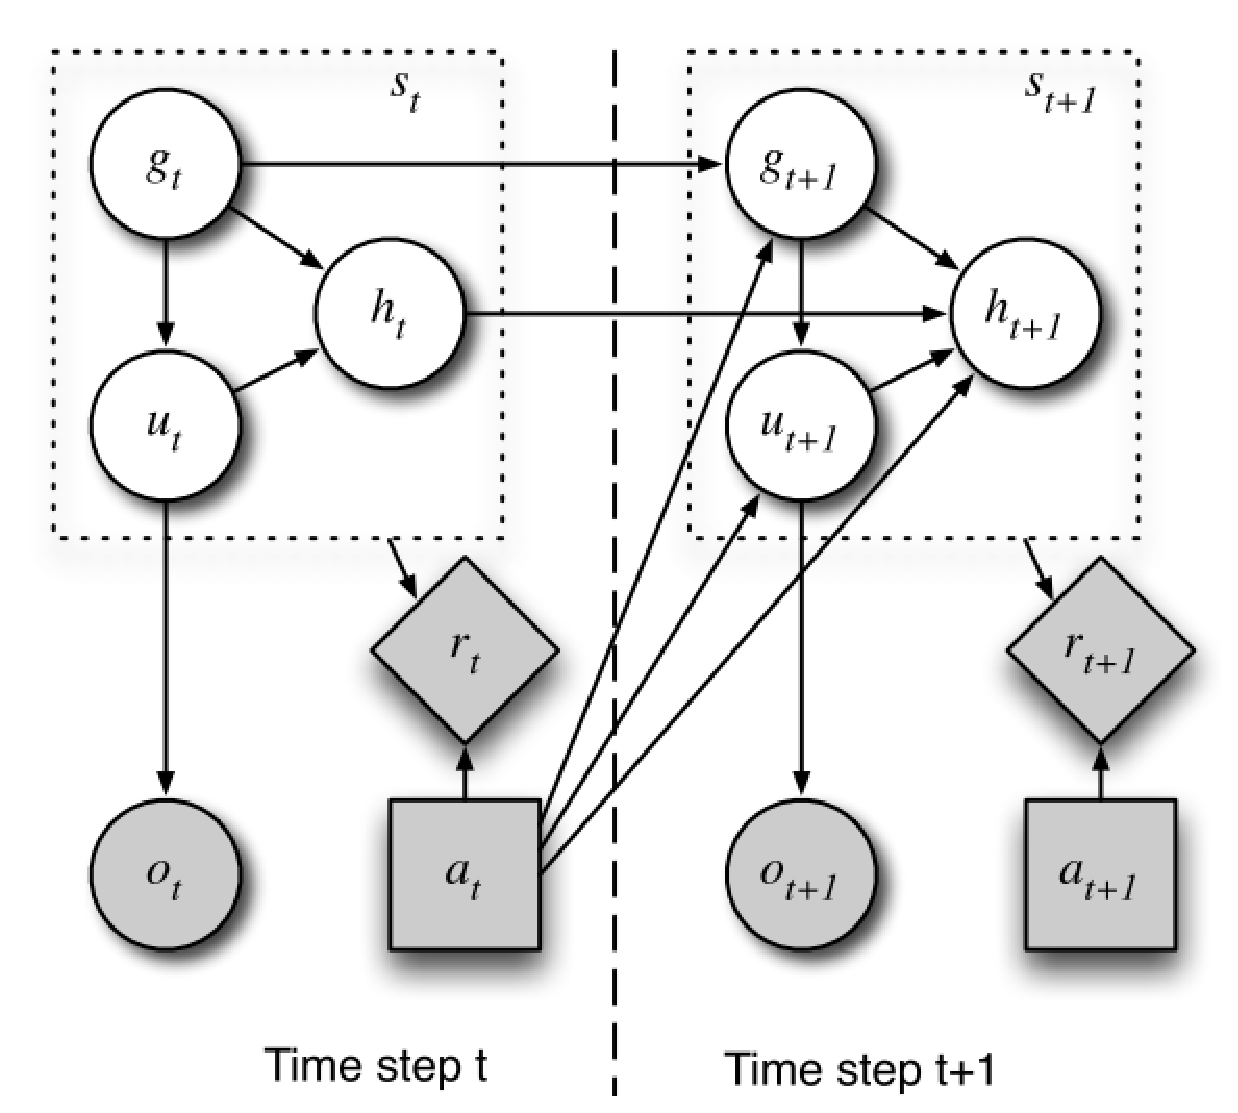
\includegraphics[width=.5\linewidth]{10_17_POMDP3}\\
  \caption{An influence diagram of a factored state POMDP}\label{fig:POMDP3}
\end{figure}

The second approach is to factor the user goal into concepts that can be spoken about by the system. This is illustrated in Figure \ref{fig:POMDP3}, which shows an example from a tourist information system, in which entities have a type, the kind of food served and an area.

The next big challenge of a POMDP-based system is the representation and estimation of the policy model. The paper presents five different methods of policy optimisation: planning under uncertainty, value iteration, Monte-Carlo optimisation, least-squares policy iteration, and natural actor-critic. These methods have been selected because all have been applied to end-to-end working dialog systems.

Another problem is also mentioned in the previous paper summaries of the MDP-based approaches: learning directly from corpora is problematic, because an interactive environment is necessary. One solution is to build a model of the user that can interact directly with a dialog system, and which can itself be trained on corpora. In a real system the dialog manager only has access to a noisy observation, so an error model is needed as well as a user model.

The following three sections presents some more advanced techniques for dialogue model parameter optimisation, fast training, user adaption, and discusses some real-world systems and applications. Finally, the paper discusses the current evaluation methods of SDS. Evaluation of SDS typically falls into one of 3 testing regimes: testing with some form of simulated user, testing with paid subjects, and testing within a live deployed system.

Remark: I am not very familiar with the POMDP approach, so some of the technical details mentioned in the paper are still not very clear to me. Intuitively, POMDP should have better performance than MDP (but also harder to train). I think it is also possible to combine it with the deep learning techniques, such as representing the transition probabilities with a neural network approximately. 